\documentclass{article}


\setcounter{tocdepth}{5}
\usepackage[subpreambles=true]{standalone}
\usepackage[utf8]{inputenc}
\usepackage[english]{babel}

\usepackage{import}
\usepackage{hyperref}
\usepackage[toc]{glossaries}
\usepackage{lscape}
\usepackage{pdfpages}
\usepackage{graphicx}
\usepackage{listings}
\usepackage{color}

\definecolor{dkgreen}{rgb}{0,0.6,0}
\definecolor{gray}{rgb}{0.5,0.5,0.5}
\definecolor{mauve}{rgb}{0.58,0,0.82}

\lstset{
    frame=tb,
    language=Java,
    aboveskip=3mm,
    belowskip=3mm,
    showstringspaces=false,
    columns=flexible,
    basicstyle={\small\ttfamily},
    numberstyle=\color{gray},
    keywordstyle=\color{blue},
    commentstyle=\color{dkgreen},
    stringstyle=\color{mauve},
    breaklines=true,
    breakatwhitespace=true,
    numbers=left,
    stepnumber=1,
    % numbersep=5pt,
    tabsize=2
}

% Define variables for the "\maketitle" command
\title{Leistungsnachweis im Fach Programmierung 1}
\date{2020-12-07 - 2020-01-17}
\author{Maximilian von Hohenbühel \\ Fabian Cieslik}
% Define the glossary
\makeglossaries
\begin{document}
\pagenumbering{Roman}
\maketitle
\newpage
\tableofcontents % Show structure of all sections and paragraphs
\newpage

\section{Projektvorraussetzungen}
\textbf{Beschreibung:} Die Projektaufgabe besteht darin, ein einfaches Spiel zu implementieren. Die Wahl des Spiels bleibt Ihnen überlassen, beachten Sie jedoch, dass sich im Rahmen von 36 Stunden Arbeitszeit nur sehr begrenzte Spielideen auch umsetzen lassen.
\newline
\textbf{Details:} Sie programmieren ein Spiel für ein sehr eingeschränktes Display. Dieses enthält nur $24\times 48$ Bildpunkte (Pixel), d.h. 24 Reihen mit jeweils 48 Spalten. Jeder Bildpunkt kann 16 Millionen Farben annehmen, wobei die Rot, Grün und Blau-Komponente mit jeweils einem Byte angesprochen wird. Als Steuermöglichkeit stehen Ihnen vier Tasten zur Verfügung, die wie im Cursorblock üblich angeordnet sind. Es gibt nur einen Spieler. Die Zeit für eine Spielrunde sollte bei 20-30 Sekunden liegen.
\newline
Zur Ein- und Ausgabe erhalten Sie eine Klasse mit zwei Methoden:
\begin{itemize}
    \item \textit{public int getKeyboard()}
        \newline
        Liefert die vier Cursortasten der Tastatur folgende Werte zurück:
        \newline - 0 -$>$ "hoch"
        \newline - 1 -$>$ "runter"
        \newline - 2 -$>$ "links"
        \newline - 3 -$>$ "rechts"
        \newline - -1 -$>$ keine Taste
    \item \textit{public void showImage(short[] image)}
        \newline
        Zeigt ein komplettes Bild auf dem Display an, wobei der erste Wert des Arrays die Rot-Komponente des linken oben Bildpunkts ist und der letzte Wert die Blau-Komponente von 0 bis 255 des rechten unteren Bildpunktes. Das übergebene Array muss exakt $24*48*3$ Elemente haben für die 24 Zeilen, 48 Spalten und 3 Farbkomponenten pro Pixel. Das Display wird zeilenweise durchlaufen.
\end{itemize}
\textbf{Spielumfang:}
\begin{itemize}
    \item Eine \textit{interaktive Spielerfigur}
    \item Eine \textit{automatisch gesteuerte Spielerfigur}
    \item Einen Hintergrund
    \item Ein \textit{Score-System}
    \item Ein \textit{Highscore-System}
    \item Implementierungsvorgaben:
        \newline - Eine generische Klasse
        \newline - Drei davon abgeleitete Klassen (Spieler, Hintergrund, Gegner/NPC)
\end{itemize}
\newpage

\section{Idee}
\textbf{Name:}
\newline
MP - Mari proelium
\newline
\textbf{Spiel:}
\newline
Idee war es, ein Spiel zu programmieren, dass in der Vogelperspektive gespielt wird, um dem Spieler die maximale Übersicht über das Spiel zu geben, d.h. man sieht ständig die vollständige Karte.
\newline
Der Spieler steuert dabei ein Schiff, welches drei Leben besitzt und probiert so lang zu überleben wie nur möglich. Es existieren sowohl Gegner, die sich zufällig bewegen und nach jeder Runde neu erzeugt werden und Inseln, mit optionalen Häfen, die bei Eroberung sowohl dem Gegner als auch dem Spieler zugewandt sein können.
\newline
Das Spiel basiert auf dem klassischen Levelprinzip, d.h. dass alle 30 Sekunden neue Gegner auftauchen, jede dritte Runde ein weiterer Gegner erzeugt wird und man für jede überlebte Runde zusätzliche Punkte bekommt. 
\newline
Das Punktesystem wird von der Zeit, die man am Leben ist und der Anzahl der besiegten feindlichen Schiffe beeinflusst.
\newline
Die Steuerung wird auf die vier verfügbaren Tasten aufgeteilt, sodass man ohne Probleme sein Schiff steuern und zugleich auch schießen kann. Die Kollisionsinteraktionen mit feindlichen Schiffen und eventuellen Häfen wird vom System übernommen.
\newpage

\section{Beschreibung}
\textbf{Karte:}
\begin{itemize}
    \item \textbf{Darstellung}
        \newline
        Der Hintergrund der Karte ist blau gefärbt und soll das Meer/den Ozean simulieren. Auf der gesamten Karte werden jede dritte Runde fünf Inseln zufällig/randomisiert erstellt. Diese lassen sich sowohl vom Gegner als auch vom Spieler einnehmen. Diese unterstützen, in Form von einer Kanone, die auf den jeweiligen Feind schießt, den jeweiligen Besitzer. Inseln werden durch gelbe und Häfen durch braune Pixel dargestellt. Die Häfen können den Besitzer „heilen“, d.h. +1 Leben verleihen. Die Spieler und Gegner können sich auf der Karte vollständig frei bewegen.
\end{itemize}
\textbf{Spieler:}
\begin{itemize}
    \item \textbf{Darstellung}
        \newline
        Ein drei Pixel langes Schiff in grüner, gelber oder roter Farbe (Je nach Anzahl der Leben).
    \item \textbf{Fähigkeiten}
        \begin{itemize}
            \item Schussrichtung senkrecht zur Fahrtrichtung (beidseitig)
            \item 3 Leben
            \item 4x schneller als Gegner
        \end{itemize}
\end{itemize}
\textbf{Gegner:}
\begin{itemize}
    \item \textbf{Darstellung}
        \newline
        Ein drei Pixel langes Schiff in blauer, violetter Farbe (Je nach Anzahl der Leben).
    \item \textbf{Fähigkeiten}
        \begin{itemize}
            \item Schussrichtung 360°
            \item 2 Leben (jede 15. Runde +1 Leben)
            \item Werden jede Runde neu erzeugt (sofern gestorben in vorangegangener Runde)
            \item Jede 3. Runde erhöht sich die Gegneranzahl um +1
        \end{itemize}
\end{itemize}
\textbf{Insel ohne Hafen}
\begin{itemize}
    \item \textbf{Darstellung}
        \newline
        Drei mal drei große Raster in gelb.
    \item \textbf{Fähigkeiten}
        \begin{itemize}
            \item Kugeln werden von Inseln geblockt
            \item Kollision verursacht keinen Schaden
        \end{itemize}
\end{itemize}

\textbf{Insel mit Hafen}
\begin{itemize}
    \item \textbf{Darstellung}
        \newline
        Drei mal drei große Raster in gelb mit einem braunen Pixel als Hafen.
    \item \textbf{Fähigkeiten}
        \begin{itemize}
            \item Können eingenommen werden
            \item Können durch Zerstörung zurückerobert werden
            \item Schussrichtung 360°
            \item Geben beim Andocken jede 3. Runde +1 Leben
        \end{itemize}
\end{itemize}

\textbf{Steuerung}
\begin{itemize}
    \item ↑ Bewegung um 1 Pixel in Fahrtrichtung
    \item ← Drehung um 45° gegen den Uhrzeigersinn
    \item → Drehung um 45° im Uhrzeigersinn
    \item ↓ Schießen (beidseitig)
\end{itemize}
\textbf{Punkte:}
\begin{itemize}
    \item \textbf{Punktequellen}
\begin{itemize}
    \item Beim treffen eines Gegners
    \item Beim besiegen eines Gegners
    \item Besiegen aller gerade lebender Geger
    \item Fürs überleben einer Runde
\end{itemize}
    \item \textbf{Highscore}
        \newline
        Punkte werden in der Konsole als Highscore nach jedem Tod des Spielers ausgegeben
\end{itemize}
\newpage

\section{Programmablauf}
\begin{itemize}
    \item \textbf{Vorbereitung}
        \newline
        Es werden alle Spielnotwendigen Variablen deklariert und initialisiert. In einer \textit{Do-While} Schleife wird daraufhin gestarted um mehrere Spiele hintereinander spielen zu Können. Am Start der Schleife wird die Karte, der Spieler und die Gegner erstellt und gezeichnet und auf eine Eingabe des Benutzers gewartet. Bei Eingabe wird der Spielablauf gestartet. Nach dem Tod des Spielers wird der Punktestand ausgegeben und die Möglichkeit geboten ein neues Spiel zu Starten oder das Program zu Beenden.
    \item \textbf{Spielablauf}
        \newline
        Zuerst wird der Spieler bewegt und auf Kollisionen überprüft, danach die Gegner. Anschließend wird überprüft ob man eine Runde überlebt hat und falls ja werden die Punkte zugewiesen und neue Gegner erstellt. Alle drei Runden wird das Spiel schwerer und die Positionen der Inseln neu gewählt.
\end{itemize}
\newpage
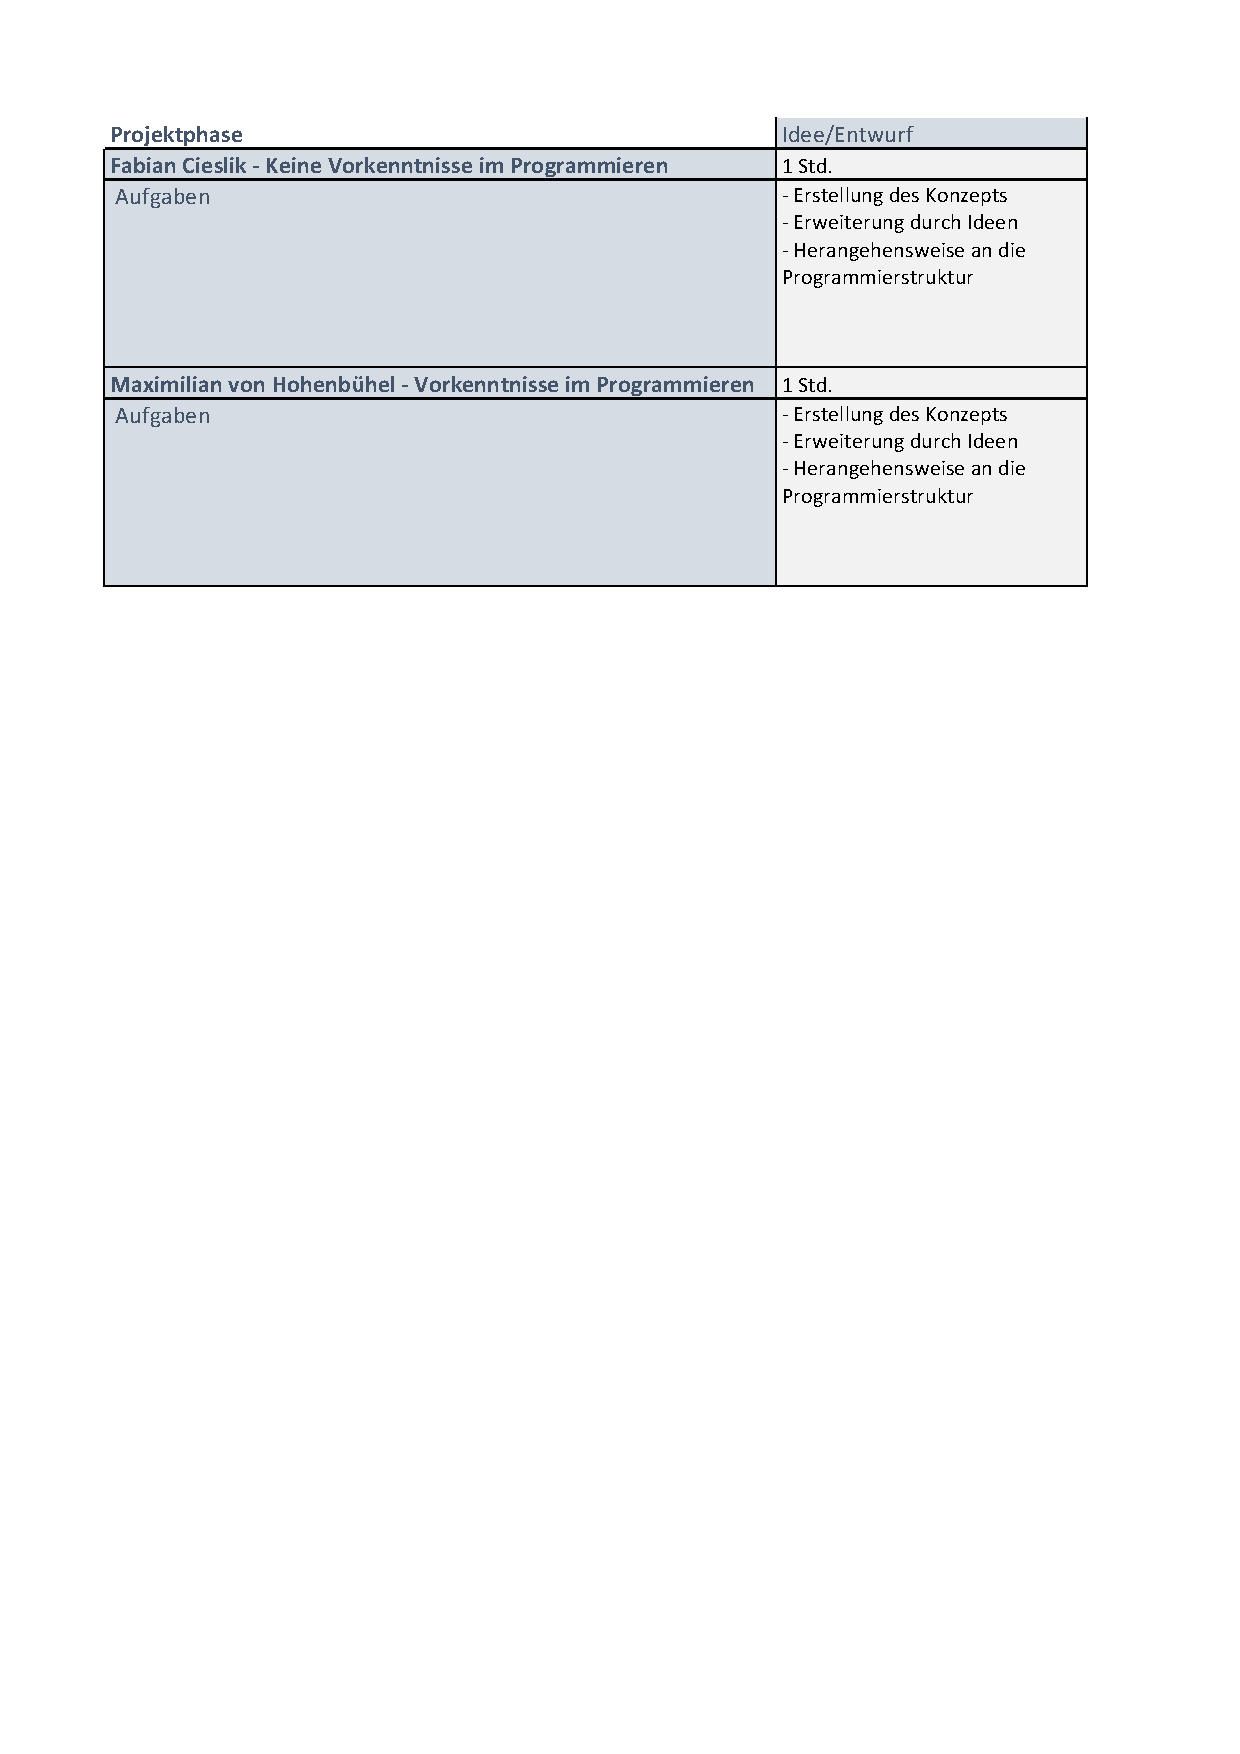
\includepdf[pages=1,landscape=true,pagecommand={\section{Arbeitsaufteilung}}]{./Stundenliste - Stundenliste.pdf}
\newpage
\section{Klassendiagramm}
Das Diagramm stellt einen groben Ausschnitt des Klassendiagramms, inklusive der Vererbung der Klassen, dar. Die ausführliche Version des Klassendiagramms befindet sich im \textit{Documentation} Ordner.
\newline

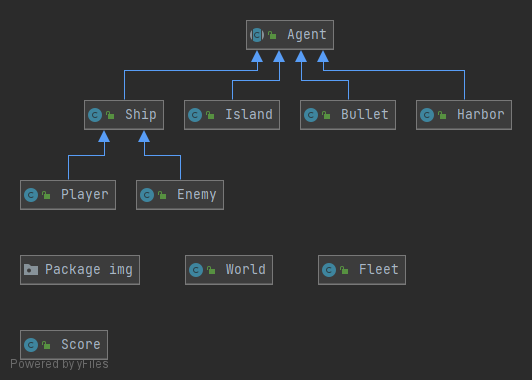
\includegraphics[width=\textwidth,height=\textheight,keepaspectratio]{./images/Rough_UML.png}
\newpage
\section{Kommentare und Zusammenfassung}

Allgemein stellt das Programmieren eines Spiels ein ideales Ende des Moduls
Programmieren 1 dar.  Die erlernten Programmierkenntnisse werden dabei
optimal abgefragt und angewendet, dadurch werden auf vielseitige Art
und Weise die Kenntnisse vertieft und erweitert.

Ein wesentlicher Kritikpunkt der individuellen Gruppeneinteilung hat sich
bei uns gezeigt. Ein Mitglied (Maximilian) ist ein bereits erfahrener bzw.
sehr fortgeschrittener Programmierer in diversen Sprachen. Das andere
Mitglied (Fabian) dagegen besitzt kaum Vorkenntnisse in diesem Bereich.
Die Schwierigkeit lag also darin, ein Spiel zu finden was beiden Ansprüchen
genügt, d.h. denjenigen ohne Kenntnisse nicht überfordert als auch
denjenigen mit fortgeschrittenen Kenntnissen unterfordert. Dieses
Ziel zu erreichen gelang leider gar nicht. Die Überforderung des Teammitglieds
ohne Kenntnisse war deutlich zu erkennen. Dies führen wir beide auf die teils
einseitigen und zu praxisfernen Übungen während des Semesters und das nicht
optimale Einleiten der Herangehensweise eines Projekts zurück. Besser/effektiver
wäre gewesen, mehrere kleinere Übungen zu jedem Teilgebiet und eine Vorlesung/ein
Skript anzubieten, das einen roten Faden von Anfang bis Ende besitzt. Die Struktur
der Vorlesung war ebenfalls nicht unbedingt von Vorteil. Diese sollte mehr Schritt
für Schritt aufgebaut sein (z.B. sollten nicht Klassen vor Zugriffsmodifikatoren
gelehrt werden). Dies hat teilweise für Verwirrung gesorgt und musste ausführlicher
vom Teammitglied mit Kenntnissen erklärt werden. Insgesamt kann man sagen, dass
wir ein einfacheres Spiel hätten wählen sollen, um die Herangehensweise an ein
solches Projekt Schritt für Schritt erklären, genügend Zeit in die Erklärung
des Stoffes investieren und die Wissens-/Kenntnislevel zu einem gewissen
Teil aneinander anpassen zu können.

Das Spiel betreffend sind wir durchaus zufrieden. Das Ergebnis hat uns
letzten Endes sehr überrascht, da wir nicht gedacht hatten, dass ein so
einfaches Spiel so Spaß machen kann. Insgesamt ist diese Idee, wie bereits
beschrieben, eine tolle Endaufgabe im Modul Programmieren 1, benötigt aber hier
und da etwas Feinschliff. Vor allem was die Gruppeneinteilung angeht, sollte man
sich etwas mehr Gedanken machen, da der Unterschied der jeweiligen Level
teilweise deutlich auseinander liegt.
\newpage
\section{Programmcode}
\textbf{Ship.java}
\lstinputlisting{../Game/src/de/thdeg/game/assets/Ship.java}
\newpage
\textbf{Agent.java}
\lstinputlisting{../Game/src/de/thdeg/game/assets/Agent.java}
\newpage
\textbf{Enemy.java}
\lstinputlisting{../Game/src/de/thdeg/game/assets/Enemy.java}
\newpage
\textbf{Fleet.java}
\lstinputlisting{../Game/src/de/thdeg/game/assets/Fleet.java}
\newpage
\textbf{Bullet.java}
\lstinputlisting{../Game/src/de/thdeg/game/assets/Bullet.java}
\newpage
\textbf{Harbor.java}
\lstinputlisting{../Game/src/de/thdeg/game/assets/Harbor.java}
\newpage
\textbf{Island.java}
\lstinputlisting{../Game/src/de/thdeg/game/assets/Island.java}
\newpage
\textbf{Player.java}
\lstinputlisting{../Game/src/de/thdeg/game/assets/Player.java}
\newpage
\textbf{GameMain.java}
\lstinputlisting{../Game/src/de/thdeg/game/assets/GameMain.java}
\newpage
\textbf{World.java}
\lstinputlisting{../Game/src/de/thdeg/game/assets/World.java}
\newpage
\textbf{Score.java}
\lstinputlisting{../Game/src/de/thdeg/game/assets/Score.java}
\end{document}
